\chapter{Združené rozdelenie pravdepodobnosti}\label{sec:joint_dist}

V predchádzajúcich kapitolách sme sa zaoberali modelovaním rozdelenia pravdepodobnosti jednotlivých náhodných premenných alebo cieľových premenných v kontexte regresie a klasifikácie. V oboch týchto prístupoch sme vychádzali prevažne z predpokladu, že modelujeme samostatnú premennú alebo závislosť jednej výstupnej premennej na vstupe. V praxi však častokrát pracujeme s viacerými náhodnými premennými súčasne, ktorých správanie môže byť navzájom ovplyvňované. Ich spoločné správanie popisuje tzv. \textit{združené rozdelenie pravdepodobnosti}.

Ak premenné modelujeme ako komponenty náhodného vektora, napríklad $\vec{X} = (X_1, X_2)$, potom znalosť ich združeného rozdelenia nám umožňuje odvodiť ďalšie dôležité vlastnosti systému – napríklad ako vyzerajú podmienené rozdelenia, marginálne rozdelenia alebo podmienená stredná hodnota jednej premennej vzhľadom k iným premenným. Tieto pojmy sú kľúčové nielen pre štatistické modelovanie ako také, ale aj pre praktické aplikácie ako sú predikcie, rozhodovania sa založené na týchto predikciách alebo celková analýza závislostí.

Presné vyjadrenie alebo odhad združeného rozdelenia je však zložitý, čo je podnecované vyšším počtom premenných. S rastúcim rozmerom vektora náhodných premenných rastie aj počet parametrov a miera závislosti, ktorú je potrebné zohľadniť. Preto sa častokrát používajú zjednodušujúce predpoklady, napríklad o nezávislosti alebo naopak špecifickej štruktúre závislosti medzi premennými.

V tejto kapitole sa zameriame na:
\begin{itemize}
  \item základy modelovania združených rozdelení, vrátane podmienených a marginálnych funkcií,
  \item rozklad združeného rozdelenia na marginálne rozdelenia a kopulovú funkciu,
  \item praktické aspekty odhadu združeného rozdelenia na základe údajov.
\end{itemize}

Konkrétne budeme v tejto kapitole pracovať so združenými rozdeleniami náhodných premenných rovnakého typu – teda buď čisto spojitými, alebo čisto diskrétnymi. Budeme rozoberať všeobecné princípy modelovania, analýzy a odhady takýchto rozdelení. Praktické príklady budú vychádzať z regresných a klasifikačných kontextov, kde sa využívajú znalosti o marginálnych a podmienených rozdeleniach. Pre ilustráciu štruktúry dát a závislostí medzi premennými využijeme nástroje popisnej štatistiky a vizualizačné techniky, ktoré sú súčasťou výstupov mnou implementovanej interaktívnej aplikácie. Táto aplikácia predstavuje aplikačnú časť tejto bakalárskej práce a poskytuje praktické vizualizačné a analytické nástroje na skúmanie združených rozdelení pravdepodobnosti, ktoré sú využité aj pri prezentácii výsledkov v tejto kapitole. Modelovanie zmesi spojitých a diskrétnych náhodných premenných, ako špecifický prípad heterogénnych štruktúr, bude predmetom samostatnej kapitoly, keďže ide o hlavnú problematiku, na ktorú sa v tejto práci chceme zamerať.


\section{Základy modelovania}\label{sec:zaklady_modelovania}

\subsection{Združená hustota pravdepodobnosti}
\label{subsec:joint_pdf}

Združené rozdelenie pravdepodobnosti pre dve náhodné premenné $X_1$ a $X_2$ môžeme opísať buď pomocou ich spoločnej distribučnej funkcie (angl. joint cumulative distribution function – CDF), alebo pomocou ďalších vhodných nástrojov v závislosti od typu premenných. 

Ak sú premenné spojité, spoločné rozdelenie opisujeme prostredníctvom \textit{združenej hustoty pravdepodobnosti} (angl. joint probability density function – PDF) $f(x_1, x_2)$, ktorá udáva pravdepodobnostnú hustotu výskytu dvojice hodnôt v danej oblasti roviny $\mathbb{R}^2$.

V prípade diskrétnych premenných sa namiesto hustoty používa \textit{združená pravdepodobnostná funkcia} (angl. joint probability mass function – PMF), ktorá každému páru hodnôt $(x_1, x_2)$ priraďuje konkrétnu pravdepodobnosť výskytu: 

\begin{equation}
p(x_1, x_2) = \mathrm{Pr}(X_1 = x_1,\, X_2 = x_2)
\end{equation}

Táto pravdepodobnosť je daná explicitne pre jednotlivé kombinácie hodnôt, pričom platí:

\begin{equation}
\sum_{x_1} \sum_{x_2} p(x_1, x_2) = 1
\end{equation}

Bez ohľadu na typ premenných platí, že združené rozdelenie poskytuje kompletný popis ich spoločného správania a tvorí základ pre odvodenie marginálnych a podmienených rozdelení, ako aj závislostí medzi premennými.

\begin{figure}[H]
    \centering
    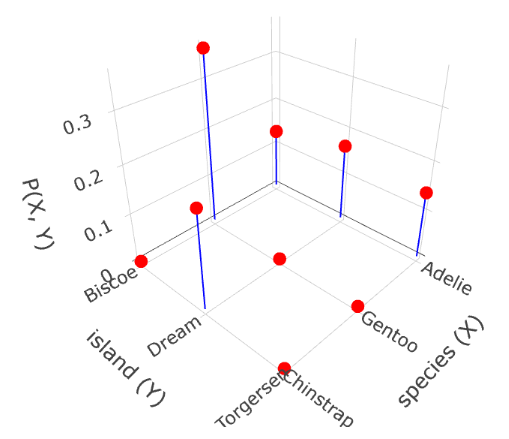
\includegraphics[width=0.7\linewidth]{SK_verzia_praca/figures/pravdeb_funk_ostrov_druhy_3D.png}
    \caption{3D znázornenie združenej pravdepodobnostnej funkcie (PMF) medzi premennými \textit{Ostrov ako miesto výskytu} a \textit{Druh} tučniakov.}
    \label{fig:miesto_druh_joint_density}
\end{figure}

Zatiaľ čo v jednorozmernom spojitom prípade nás zaujímala pravdepodobnosť výskytu náhodnej premennej v určitej oblasti na reálnej osi, v prípade dvoch spojitých premenných nás už zaujíma pravdepodobnosť, že realizácie oboch premenných spadnú do danej oblasti v rovine $\mathbb{R}^2$.

Ak $R_1 = [x_1, x_1 + dx_1]$ a $R_2 = [x_2, x_2 + dx_2]$ sú malé intervaly okolo bodu $(x_1, x_2)$, potom pravdepodobnosť, že náhodný vektor $(X_1, X_2)$ spadne do oblasti $R_1 \times R_2$, je približne:

\begin{equation}
\mathrm{Pr}(x_1 \leq X_1 \leq x_1 + dx_1,\ x_2 \leq X_2 \leq x_2 + dx_2) \approx f(x_1, x_2) \, dx_1 \, dx_2
\end{equation}

kde $f(x_1, x_2)$ je hodnota združenej hustoty pravdepodobnosti v bode $(x_1, x_2)$.

Presnejšie, pravdepodobnosť, že sa realizácie oboch premenných nachádzajú v oblasti $[a_1, b_1] \times [a_2, b_2]$, vypočítame pomocou dvojnásobného integrálu:

\begin{equation}
\mathrm{Pr}(a_1 \leq X_1 \leq b_1,\ a_2 \leq X_2 \leq b_2) = \int_{a_2}^{b_2} \int_{a_1}^{b_1} f(x_1, x_2) \, dx_1 \, dx_2
\end{equation}

Aby funkcia $f(x_1, x_2)$ bola platnou hustotou pravdepodobnosti, musí platiť:

\begin{equation}
\iint_{\mathbb{R}^2} f(x_1, x_2) \, dx_1 \, dx_2 = 1
\end{equation}

Združená hustota veľmi efektívne popisuje spoločné správanie sa dvoch spojitých náhodných premenných a tvorí základ pre ďalšie koncepty ako sú marginálne a podmienené rozdelenia.

Na nasledujúcom obrázku môžeme vidieť príklad vizualizácie združenej hustoty pravdepodobnosti homogénnej spojitej štruktúry dvoch premenných, pričom ako model výpočtu tu používame jadrové vyhladzovanie, viď ~\ref{textbf:kernel_smoothing}.

\begin{figure}[H]
    \centering
    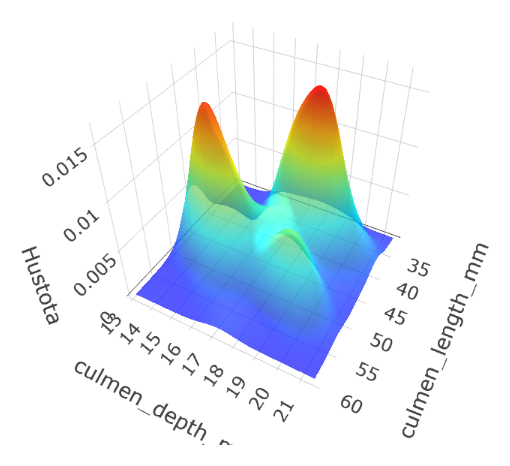
\includegraphics[width=0.7\linewidth]{hustota_hlbka_dlzka_zobaku_3D}
    \caption{3D znázornenie združenej hustoty pravdepodobnosti (PDF) medzi premennými \textit{Hĺbka zobáku} a \textit{Dĺžka zobáku} tučniakov.}
    \label{fig:zobak_joint_density}
\end{figure}


\section{Rozklad - marginálne rozdelenia + kopula}\label{sec:rozklad_kopule}
\section{Odhad}\label{sec:odhad}